% Uncomment this to make slides with overlays:
\documentclass[slides]{beamer}

% Uncomment these (but comment the above \documentclass line) to make handouts:
%\documentclass[handout]{beamer}

% Uncomment these to have more than one slide per page
%\usepackage{pgfpages}
%\pgfpagesuselayout{2 on 1}[border shrink=5mm]
%\pgfpageslogicalpageoptions{1}{border code=\pgfusepath{stroke}}
%\pgfpageslogicalpageoptions{2}{border code=\pgfusepath{stroke}}

\usepackage[]{graphicx, color, hyperref}

\mode<presentation>
{
	%\usetheme[secheader]{Boadilla}
	%\usecolortheme[rgb={.835, .102,.169}]{structure}  
	\usetheme[width= 0cm]{Goettingen}
	%\setbeamercovered{transparent}
}
\setbeamertemplate{navigation symbols}{}
\setbeamertemplate{footline}[frame number]

\definecolor{blue2}{rgb}{0.278,0.278,0.729} 
\newcommand{\blue}[1]{\textcolor{blue2}{#1}}
\newcommand{\white}[1]{\textcolor{white}{#1}}
\newcommand{\red}[1]{\textcolor{red}{#1}}
\newcommand{\xbar}{\overline{x}}
\newcommand{\ybar}{\overline{y}}
\newcommand{\phat}{\widehat{p}}
\newcommand{\prob}{\mbox{Pr}}
\newcommand{\E}{\mathbb{E}}
\newcommand{\Var}{\mbox{Var}}
\newcommand{\cp}{\oplus}
\newcommand{\cm}{\circleddash}


\title{Lecture 31: $t$ Distribution for Difference of Two Means}
\author{Chapter 5.4}
\date{}


\begin{document}
%------------------------------------------------------------------------------
\begin{frame}
\titlepage
\end{frame}
%------------------------------------------------------------------------------



%%-------------------------------------------------------------------------------
%\begin{frame}
%\frametitle{Previously... Conditions/Assumption for Using t Dist'n}
%The key situation to use the $t$ distribution is when you have a \blue{small sample}.
%
%\begin{itemize}
%\item \blue{Independence of observations}: To ensure this, either
%\begin{itemize}
%\item collect a simple random sample that is less than 10\% of the population
%\item or if it was an experiment or random process check that each observation was independent
%\end{itemize}
%\item \blue{Observations come from a nearly normal distribution}:  This second condition is difficult to verify with small data sets:
%\begin{itemize}
%\item take a look at a plot of the data for obvious departures from the normal model
%\item consider whether any previous experiences alert us that the data may not be nearly normal
%\end{itemize}
%\end{itemize}  	
%\end{frame}
%%-------------------------------------------------------------------------------
%
%
%
%%-------------------------------------------------------------------------------
%\begin{frame}
%\frametitle{Previously... Confidence Intervals and $t$-Test}
%
%We have the same two methods for inference as in Chapter 4, but:
%\begin{enumerate}
%\item Confidence intervals:  Now we use $t^*_{df}$ instead of $z^*$
%\[
%\left[\xbar - t_{df}^* SE, \mbox{  }\xbar + t_{df}^* SE\right] = 
%\left[
%\overline{x} - t_{df}^* \times\frac{s}{\sqrt n}, \mbox{  }
%\overline{x} + t_{df}^* \times\frac{s}{\sqrt n}
%\right]
%\]
%\item Hypothesis testing:  Now we use the \blue{t-test}
%\[
%t = \frac{\overline{x}-\mbox{null value}}{SE}
%\]
%using the t-table on page 410 (instead of z-table) for $df=n-1$
%\end{enumerate}
%
%\end{frame}
%%-------------------------------------------------------------------------------




%------------------------------------------------------------------------------
\begin{frame}[fragile]
\frametitle{Question for Today}

In Chapter 5.2 we asked:  Did men ($n_m=45$) run faster than women ($n_w=55$) in the Cherry Blossom Race?
\begin{center}
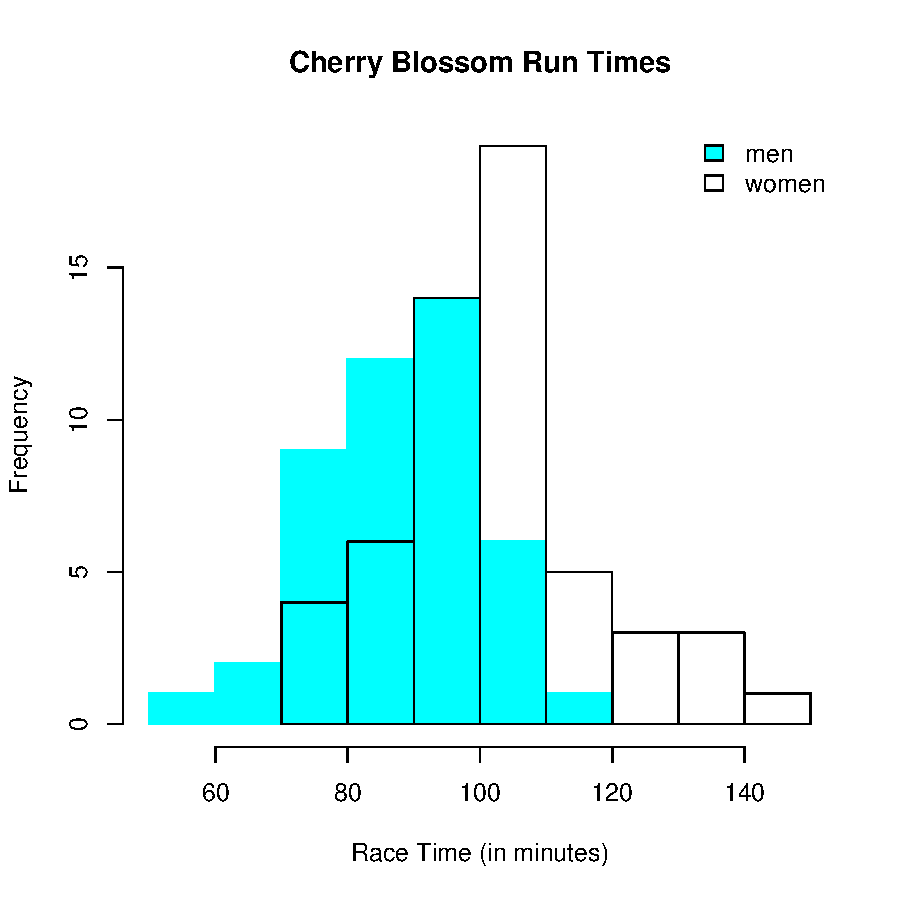
\includegraphics[width=0.4\textwidth]{figure/race.pdf}
\end{center}

\pause What can we say about $\mu_1 - \mu_2$ when $n_1$ and $n_2$ are both small?

\end{frame}
%------------------------------------------------------------------------------




%------------------------------------------------------------------------------
\begin{frame}[fragile]
\frametitle{Components}


Similarly to \blue{one-sample $t$-tests}, now we use the \blue{two sample $t$-test}: 

\begin{enumerate}
\pause \item The point estimate of $\mu_1 - \mu_2$ is $\xbar_1 - \xbar_2$
\pause \item The standard error of the sampling distribution
\[
SE_{\xbar_1 - \xbar_2} = \sqrt{\frac{s_1^2}{n_1} + \frac{s_2^2}{n_2}}
\]
\pause \item Confidence intervals using $t^*_{df}$
\pause \item Hypothesis tests using $t$-statistic
\end{enumerate}


\end{frame}
%------------------------------------------------------------------------------



%------------------------------------------------------------------------------
\begin{frame}[fragile]
\frametitle{Components}

But what degrees of freedom $df$ do we use?  

\vspace{0.25cm}

\pause The true formula for degrees of freedom is
\[
df = \frac{(s_1^2/n_1 + s_2^2/n_2)^2}{(s_1^2/n_1)^2/(n_1-1) + (s_2^2/n_2)^2/(n_2-1)}
\]

\pause Rather, for this class, use the smaller of $n_1$ and $n_2$ minus 1 i.e.
\[
\min(n_1, n_2) - 1
\]

\end{frame}
%------------------------------------------------------------------------------



%------------------------------------------------------------------------------
\begin{frame}[fragile]
\frametitle{Conditions of Two Sample $t$-Test}

\begin{itemize}
\item Both samples meet the conditions for using the $t$ distribution
\begin{itemize}
\pause \item Sample observations are nearly normal
\pause \item Sample observations are independent within their respective populations
\end{itemize}
\pause \item The two \blue{samples} are independent
\end{itemize}

\end{frame}
%------------------------------------------------------------------------------




%------------------------------------------------------------------------------
\begin{frame}[fragile]
\frametitle{Pooled Standard Deviation Estimate}
Say however, you suspect both populations have similar true population standard deviations $\sigma_1=\sigma_2=\sigma$.  

\pause \vspace{0.5cm}

If so, we can leverage this fact to make the $t$ distribution approach slightly more precise.


\end{frame}
%------------------------------------------------------------------------------



%------------------------------------------------------------------------------
\begin{frame}[fragile]
\frametitle{Pooled Standard Deviation Estimate}
The pooled standard deviation estimate is
\[
s^2_{pooled} = \frac{s_1^2\times(n_1 -1) + s_2^2 \times(n_2 -1)}{n_1 + n_2 - 2}
\]

\vspace{0.25cm}

\pause  So use $s^2_{pooled}$ instead of $s_1^2$ and $s_2^2$ in $SE$:
\[
SE_{\xbar_1 - \xbar_2} = \sqrt{\frac{s_1^2}{n_1} + \frac{s_2^2}{n_2}}
= \sqrt{\frac{s^2_{pooled}}{n_1} + \frac{s^2_{pooled}}{n_2}} =
\sqrt{s^2_{pooled}\left(\frac{1}{n_1} + \frac{1}{n_2}\right)}
\]


\end{frame}
%------------------------------------------------------------------------------



%------------------------------------------------------------------------------
\begin{frame}[fragile]
\frametitle{Pooled Standard Deviation Estimate}

You can think of $s^2_{pooled}$ as being very close to a \blue{weighted average} of the two sample standard deviations:

\begin{eqnarray*}
\pause s^2_{pooled} &=& s_1^2 \times\frac{n_1 - 1}{n_1 + n_2 - 2} + s_2^2 \times  \frac{n_2 - 1}{n_1+n_2-2}\\
\pause \mbox{close to} &\approx& s_1^2 \times\frac{n_1}{n_1 + n_2} + s_2^2 \times  \frac{n_2}{n_1+n_2}
\end{eqnarray*}

\vspace{0.5cm}

\pause The $-1$ and $-2$ are \blue{degrees of freedom} corrections.  

\end{frame}
%------------------------------------------------------------------------------


%% SHOW THIS NEXT TIME
%%------------------------------------------------------------------------------
%\begin{frame}[fragile]
%\frametitle{Pooled Standard Deviation Estimate}
%
%So say $n_1=10$ and $n_2=20$, then 
%\begin{eqnarray*}
%s^2_{pooled} &\approx& s_1^2 \times\frac{10}{10 + 20} + s_2^2 \times  \frac{20}{10+20}\\
%&\approx& s_1^2 \times\frac{1}{3} + s_2^2 \times  \frac{2}{3}\\
%\end{eqnarray*}
%
%
%\end{frame}
%%------------------------------------------------------------------------------


%------------------------------------------------------------------------------
\begin{frame}[fragile]
\frametitle{Pooled Standard Deviation Estimate}
\blue{Benefits}:  If $\sigma$'s are equal, we have more precise model of the sampling distribution of $\xbar_1 - \xbar_2$

\vspace{0.5cm}

\pause \blue{Caveats}:  Only pool when background research/intuition indicates the population $\sigma_1$ and $\sigma_2$ of the two groups are nearly equal.  
\end{frame}
%------------------------------------------------------------------------------







\end{document}










